\chapter{The Level 1 trigger upgrade} % 

\section{Legacy System and Stage 1 Upgrade}
The Level 1 trigger is designed to filter from $40MHz$ to $\mathcal{O}(100kHz)$ to allow processing by the high level trigger while keeping high acceptance for interesting events. This has worked well at previous luminosities up to $0.7\times10^{34} cm^{-2}s^{-1}$. However, with the upgrade the maximum luminosity will increase to $1.6\times10^{34} cm^{-2}s^{-1}$. The L1 trigger system takes no tracking information and so must rely on only information from the electromagnetic (ECAL) and hadronic (HCAL) calorimeters \cite{gct}. The trigger system takes input from  trigger towers (TT) corresponding to $5\times5$ ECAL crystals \footnote{Each TT corresponds to $0.087\times0.087$ in $\Delta\eta\times\Delta\phi$. For simplicity $\eta$ and $\phi$ units of one trigger tower are used in the remainder of this report.} and an identical area in the HCAL. The extent of the calorimeter is $56\times72$. The legacy Global Calorimeter Trigger (GCT) is designed to find jets, electrons and photons and to compute global energy sums. Trigger towers are grouped into $4\times4$ blocks and features are found using algorithms described in \cite{gctalgo}. Due to hardware limitations the detector is split into 16 regions which are processed by the Regional Calorimetric Trigger (RCT) to form candidates and sum energies. The RCTs must share information to account for features which occur at boundaries between them. The RCTs are then combined in the GCT which computes global quantities and sorts the jets before deciding on whether to store the event. The firmware and algorithms used by this system will be upgraded for the beginning of run 2. This will allow pileup subtraction and better jet and particle identification at L1. This is the stage 1 upgrade. 
\section{Stage 2 Calorimetric Trigger Upgrade}
To process the data with global algorithms there is a trade off between granularity and the sharing of data. An alternative to this is the Time Multiplexed Trigger (TMT) \cite{rose}. This splits the data by time rather than detector region. This works by a two layer system. In layer 1, data is received for different regions of the detector on pre-processor boards. These are then combined in a single main processing board in layer 2 (the Imperial MP7 FPGA). Each time slice is then given to a different board until the first has finished processing the information to avoid dead time. The time multiplexing means that each event may be wholly processed on one board without loss of granularity. Jet and particle identification algorithms may thus use information on the level of trigger tower granularity. There are numerous further technical improvements over the GCT outlined in \cite{rose}. The results shown below concern studies for optimal jet algorithms using a trigger based on such a system. This is the stage 2 trigger upgrade and will run alongside the stage 1 upgrade in the commissioning stage (2015) and should become the trigger in 2016. The comparison between legacy and TMT is shown in figure \ref{tmux}.
\begin{figure}
\centering
    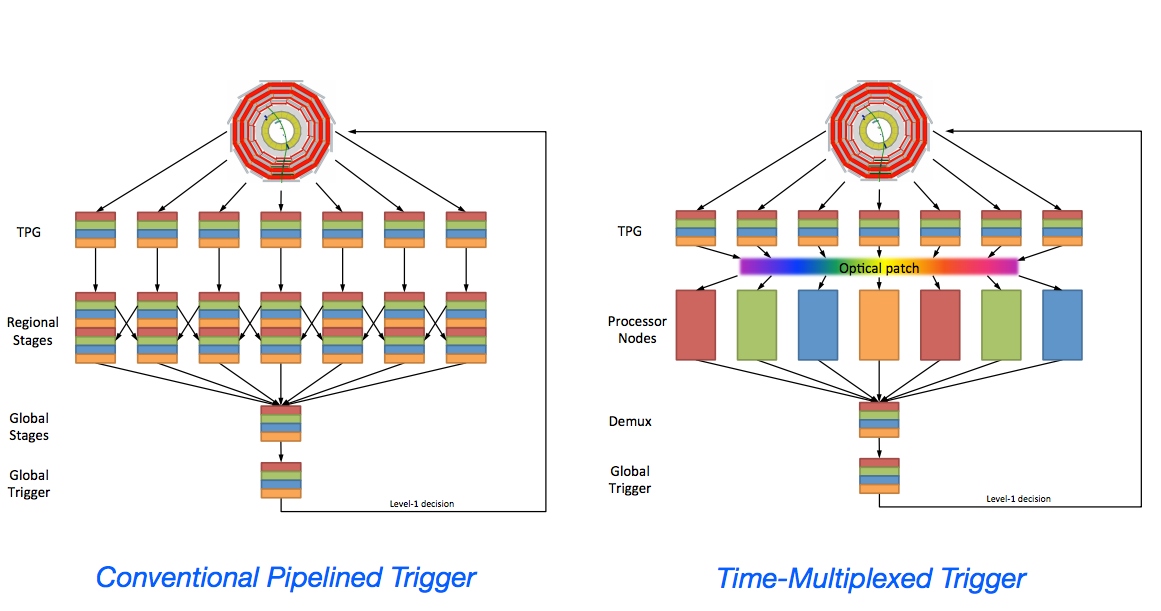
\includegraphics[width=0.9\textwidth]{././Figures/triggerUpgrade/tmux}
  \caption{Comparison of the legacy and upgrade trigger systems where colour indicates the time slice \cite{JBrooke}. The TPG is the Trigger Primitive Generator from the ECAL and HCAL.}
  \label{tmux}
\end{figure}

\section{Jet Algorithm}
\label{algo}
The focus of the results in this report will be on studies for jet definitions and pileup subtraction algorithms for the stage 2 trigger. The legacy jet algorithm is described in \cite{gctalgo}. At stage 2 the TMT allows the granularity to be significantly increased compared to the legacy system (the cells used to make the jets will reduce from $4\times4$ towers to single towers). The algorithm must change to take advantage of this. Additionally, the increase in energy to $13TeV$ will mean jets are  boosted and therefore smaller in size. To account for this at level one the cone size should be decreased. The algorithm presented here uses a cone size of $9\times9$ (compared to $12\times12$ for the GCT). This corresponds to the decrease in jet size for the HLT - from $R=0.5$ to $R=0.4$ for the anti $k_T$ jet radius parameter \cite{Antik_t}. Additionally, the boost for jets from the primary vertex means most of their energy is likely to be in the central (seed) tower which should define their direction. The algorithm is thus as follows: each trigger tower in turn is taken as the candidate. The towers in the 4 surrounding rings (or up to the edge in $\eta$) are then compared to the seed tower using the mask shown in figure \ref{mask}. If the comparison is true for any tower then the seed is vetoed and the next tower is checked. The mask is designed to be unambiguous for towers of equal energy. If a seed is not vetoed then a jet is defined at that tower position with $p_T$ given by the total energy of the towers.   
\begin{figure}
\centering
    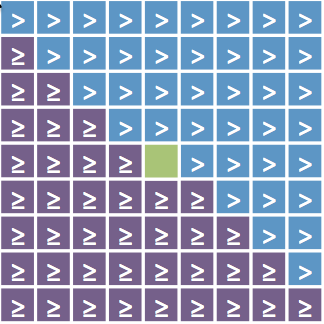
\includegraphics[width=0.5\textwidth]{./Figures/triggerUpgrade/mask.png}
  \caption{Nine by nine mask used to define jets}
  \label{mask}
\end{figure}
The two main problems with this algorithm are that sufficiently close jets will appear as a single jet and that energy may be lost if a tower that vetoes another is itself vetoed by a tower sufficiently far away not to include the far tower's energy. The first case is common to all jet algorithms with a fixed cone size, but as the energy is not lost, the single jet or total energy will almost certainly be enough to trigger. Despite this a quality bit adapted from the idea of n-subjetiness \cite{nsub} is under investigation. The lost energy from chain vetos is found to be a small (~0.1\%) inefficiency.

\section{Pileup Subtraction}
\subsection{Pileup}
The luminosity of the LHC will be increased in the upgrade to a maximum of $L = 1.4\times10^{34} cm^{-2}s^{-1}$. The easiest way to increase luminosity while maintaining stability is to use large, but widely separated, proton bunches \cite{PUform}. However, for the detector this means increased number of primary vertices (pileup) at the collision point. The average number of interactions per bunch crossing is given in equation \ref{pu}.

\begin{equation}
\langle N_p \rangle = \sigma L \tau_b
\label{pu}
\end{equation}

where $\langle N_p \rangle$ is the average number of interactions, $\sigma$ is the cross section and $\tau_b$ is the bunch spacing. At the end of run 1 with $8 TeV$ ($\sigma = 71.5mb$), $\tau_b = 50ns$ and $L = 0.75\times10^{34} cm^{-2}s^{-1}$ gave $\langle N_p \rangle\simeq27$. After LS1 the luminosity and $\sigma$ gain (to $76mb$) will increase this to $\langle N_p \rangle\simeq40$. 
\subsection{Effect of Pileup}
The majority of pileup events are low energy QCD processes which will appear as randomly distributed energy in the calorimeter region (about 1 GeV per unit area). This pileup can have two detrimental effects for the L1 trigger. Firstly, when the pileup is evenly distributing the energy of the real jets is slightly increased, thus artificially increasing the total transverse energy. The second problem occurs when the pileup is randomly clustered - significantly boosting a single jet or forming fake jets. Due to the imperfect response of the detector and profile of the pileup these effects may be dependent on $\eta$. In order to trigger only on hard events the effect of the pileup must be mitigated (subtracted). In this report two example methods of pileup subtraction (global $\rho$ and donut) will be discussed.
\subsection{Global $\boldsymbol{\rho}$}
If the detector response is assumed to be approximately $\eta$ independent then one may use an event based pileup subtraction. In the case of global $\rho$ first all the jets are reconstructed using the algorithm in \ref{algo}. The jets are then ranked in order of energy density $\rho$ where for jet $i$, $\rho^i$ is defined in equation \ref{rho}.
\begin{equation}
\label{rho}
\rho^i = \frac{p^i_{T}}{A_i} 
\end{equation}
where $A_i$ is the area of the jet. The median $\rho$ ($\rho^m$) of the jets is then taken as the estimator of the pileup energy density in the event \cite{jetarea}. All jets are in the event then reduced in energy by $\rho^m \times A^i$ and those with $p_{T}^i < \rho^m \times A_i$ taken to be pileup and removed. The correlation of this parameter with the number of interactions is shown in figure \ref{rhonint}. This method has the advantage of being stable against fluctuations, however, local effects are not considered and there is an inherent under-subtraction bias in the event as the pileup jet $p_{T}$ forms a bound on the energy subtracted per jet.
\subsection{Donut Subtraction}
\begin{figure}
\centering
    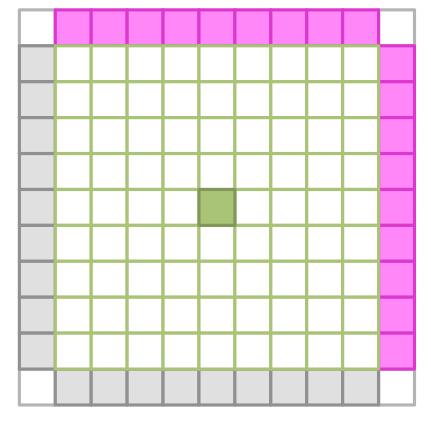
\includegraphics[width=0.5\textwidth]{./Figures/triggerUpgrade/donut}
  \caption{Donut ring for pileup estimate. Neglecting the corners the pileup energy density is taken as that in the middle two strips.}
  \label{mask}
\end{figure}  
Donut subtraction takes advantage of the area around each jet to make a local subtraction. The energy contribution from the jet is expected to be negligible by the outside ring ($\Delta R^2\simeq 0.2$) \cite{jetmet}. Taking the four strips around the jet as shown in figure \ref{donutnint} they are ordered in energy and the pile up energy density ($\rho_d$) is taken as the energy of the middle strips divided by their area ($A_d$). This energy density is then subtracted from the jet as for global $\rho$. The dependence of $\rho_d$ on number of vertices is shown in figure \ref{donutnint}. The highest strip is neglected to remove the contamination of nearby jets and the lowest to account for edge effects. Unlike global, donut subtraction allows local dependence of pile up to be taken into account, however, it is susceptible to fluctuations as the sampling region is small.

An additional method to remove pure pileup jets is to require a seed threshold. This takes advantage of the fact that pileup jets have flatter topologies. This is because, unlike the jets from the primary vertex, they are made from clusters of uniform pileup. A threshold on the seed tower can thus reduce the rate of pileup while maintaining efficiency. Donut subtraction may then be performed to correct the remaining jets. A seed threshold is not possible before the global $\rho$ calculation as this relies on lower $p_{T}$ jets for the pileup estimation. Optimising the seed (perhaps as a function of $\eta$) is under way, however, a threshold of 2.5GeV (5 level one units) was chosen as a benchmark.

\begin{figure}
\hfill
\subfigure[Global $\rho$ \label{rhonint}]{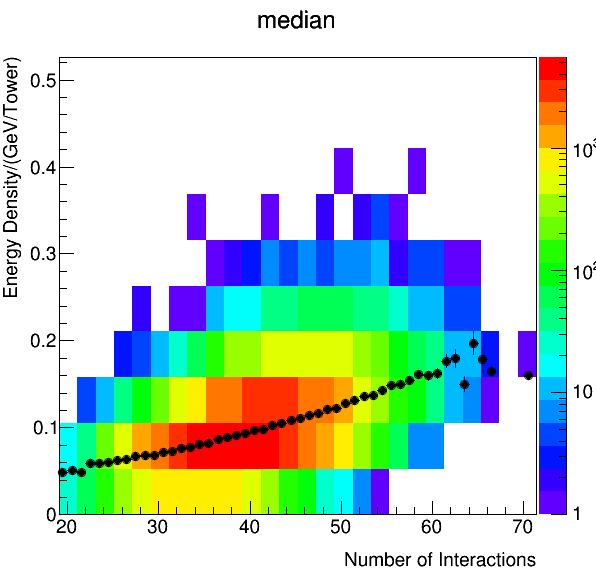
\includegraphics[width=7cm]{./Figures/triggerUpgrade/strips_median}}
\hfill
\subfigure[Donut Subtraction\label{donutnint}]{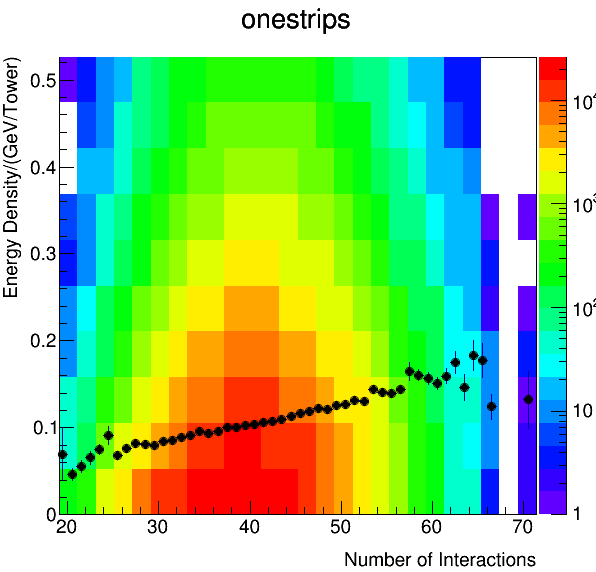
\includegraphics[width=7cm]{./Figures/triggerUpgrade/strips_onestrips}}
\hfill
\caption{Dependence on the number of interactions of the two pileup subtraction regimes studied.}
\end{figure}

\section{Jet Algorithm}
\subsection{Efficiencies}
In order to test the jet finding algorithm the first study that must be undertaken is into the matching efficiency of the L1 jets to generator level quantities (gen jets). A simulated sample of $t\bar{t}$ pairs was used\footnote{In this report all simulated samples used have conditions of $13TeV$ collisions with bunch spacing $50ns$. The pileup is gaussian distributed around $40$ interactions per bunch crossing}. The gen jets are made by running the anti-kt algorithm with radius parameter $R=0.4$ on generator level quantities. The gen jet is said to be matched if it is within ${\Delta R}^2<33$ of a L1 jet (the greatest extent of the L1 jet). The matching efficiency for alljets and the fourth jet is shown in figure \ref{match}. It can be seen that the efficiency after pileup subtraction/seed drops at low $p_T$. This motivates a cut at $30GeV$ for the calculation of energy sums. Inefficiencies at high $p_T$ are caused by the `chain veto', however, the jet algorithm guarantees there is always a comparable or higher jet in the event in such cases. The performance compared to GCT is seen to be greatly improved.  
\begin{figure}
\hfill
\subfigure[All jets\label{fig:label:alljet}]{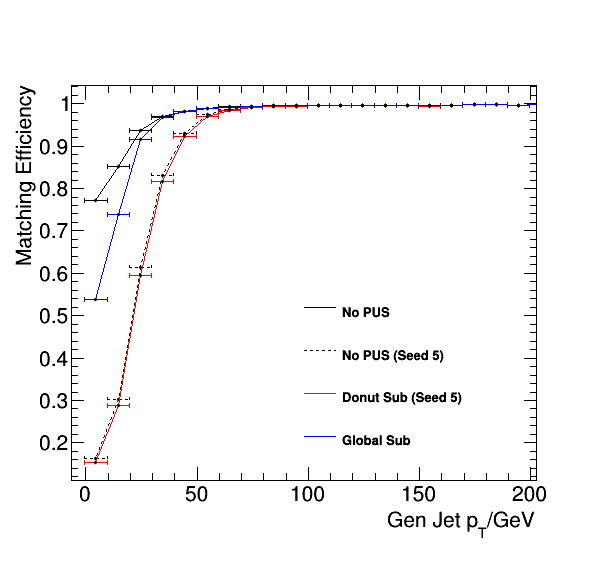
\includegraphics[width=6.9cm]{./Figures/triggerUpgrade/alljet}}
\hfill
\subfigure[4th jet\label{fig:label:jet4}]{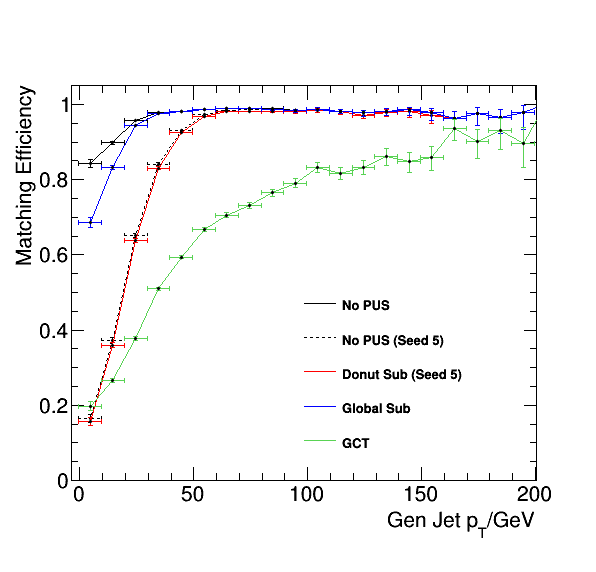
\includegraphics[width=7cm]{./Figures/triggerUpgrade/jet4}}
\hfill
\caption{Matching efficiencies for jets showing effect of seed and pileup subtraction at low energies. In \ref{fig:label:jet4} a comparison with the GCT is shown.}
\label{match}
\end{figure}
\subsection{Calibration}
The energy of the L1 jets is calibrated using generator level quantities. The scheme for calibration is outlined in \cite{l1jet_calibration}. The calibration is carried out in bins of $\eta$ to account for the difference in performance of the detector. Using a QCD sample, the response (defined as $p^{L1}_{T}/p^{gen}_{T}$) and $p^{L1}_{T}$ are plotted against $p^{gen}_{T}$ and fitted. The fits are then plotted against each other and the result itself fitted. This gives calibration factors as a function of $p^{L1}_{T}$.  Where the matching efficiency is low it is not possible to fit and so the calibration has a lower bound on $p_T$. This was found to occur at $30GeV$. An upper bound is defined by where the fits become statistically limited. This was found to occur at $300GeV$. If the fit is well defined the calibration factor should flatten with increasing $p_T$ and so higher $p_T$ jets may still be calibrated by continuing the fit. The calibration factors change depending on the pileup subtraction regime. In figure \ref{calib} the effect of the calibration is shown.   

\begin{figure}
\centering
    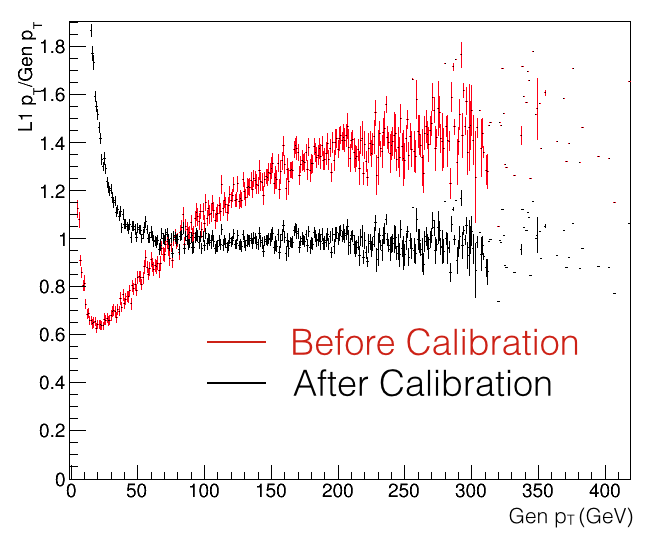
\includegraphics[width=7cm]{././Figures/triggerUpgrade/calibration}
  \caption{Effect of calibration on donut subtracted jets. At the limit of calibration ($30GeV$) the difference for the calibrated sample is around $10\%$.}
  \label{calib}
\end{figure}
\section{Pileup Subtraction}

\subsection{Resolution Dependence on Number of Interactions}
In this section plots are shown for the highest $|\eta|$ bin as the detector performance is expected to worsen with larger $|\eta|$ and so pileup subtraction will have the largest effect. The first test of any pileup subtraction scheme is the effect on the resolution. In an ideal post pileup subtraction scenario this will be flat as a function of the number of interactions. In figure \ref{fig:label:resolution1} this is plotted for a particular $p^{gen}_T$ and $\eta$ bin. It can be seen that the response flattens for both pileup subtraction regimes. This is summarised in \ref{fig:label:resolution2} where the gradient from the fit to the resolution plot is shown to reduce after pileup subtraction for a range of $p^{gen}_T$ bins.  
\begin{figure}
\hfill
\subfigure[\label{fig:label:resolution1}]{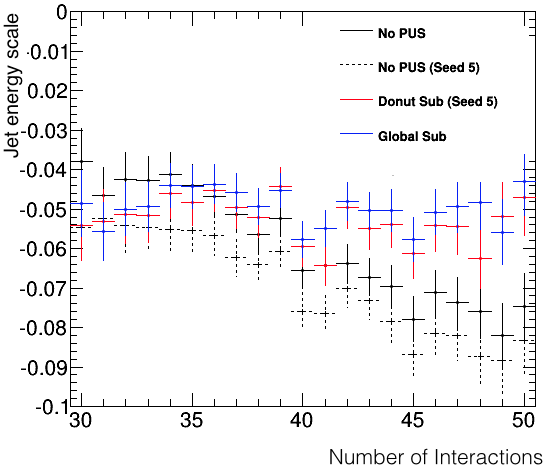
\includegraphics[width=6.8cm]{./Figures/triggerUpgrade/resolution}}
\hfill
\subfigure[\label{fig:label:resolution2}]{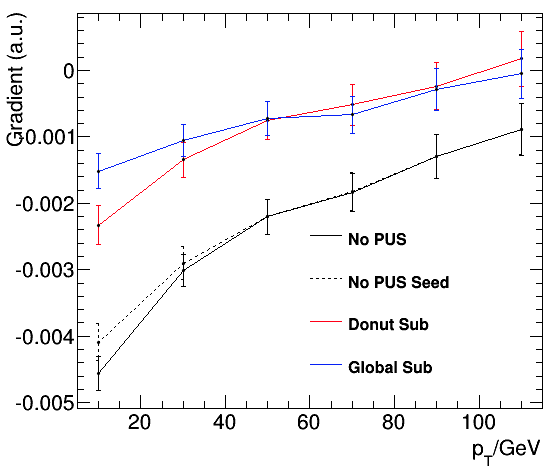
\includegraphics[width=7.1cm]{./Figures/triggerUpgrade/p1eta_14to28_calib_fits}}
\caption{In \ref{fig:label:resolution1} response versus number of interactions is shown for a particular eta bin showing the response flattens after pileup subtraction. In \ref{fig:label:resolution2} the fit gradient for different $p^{gen}_{T}$ bins is shown.}
\label{fig:label:resolution}
\end{figure}
\subsection{Rates and Efficiencies}
The rate is defined as the number of background events passing selection per second. The nominal rate for the L1 trigger is $\mathcal{O}100kHz$. The efficiency is then the proportion of signal events which trigger. To evaluate this a cut is made on the gen jets ($50GeV$). The proportion of these events with a corresponding matched L1 jet over a threshold then defines the efficiency at that threshold.  For the trigger, the key test is to see that the efficiency for signal may be maintained while reducing the background rate. For the background a pure pileup sample was used while the $t\bar{t}$ samples was used for signal. In figure \ref{fig:label:ratejet1} the rate is shown for the leading jet. The performance compared to the GCT is shown to be improved. The seed cut appears to have the largest effect in reducing the rate as global is shown to be comparable to no pileup subtraction. Figure \ref{fig:label:ratenvtx} shows the evolution of the rate with the number of interactions. GCT shows the largest dependence, as expected, while for stage 2 pileup subtraction is shown to decrease this dependence. Applying donut subtraction appears to increase the rate compared to applying a seed alone. This may be due to contamination causing over subtraction. The calibration will then bring the energy above the seed. Finally, in figure \ref{fig:label:rateeff} the rate is shown against efficiency for the lead jet. The seed is shown to be comparable to global subtraction alone while applying donut subtraction worsens the performance. This may again be due to contamination.
\begin{figure}
\hfill
\subfigure[Jet 4 Rate\label{fig:label:ratejet1}]{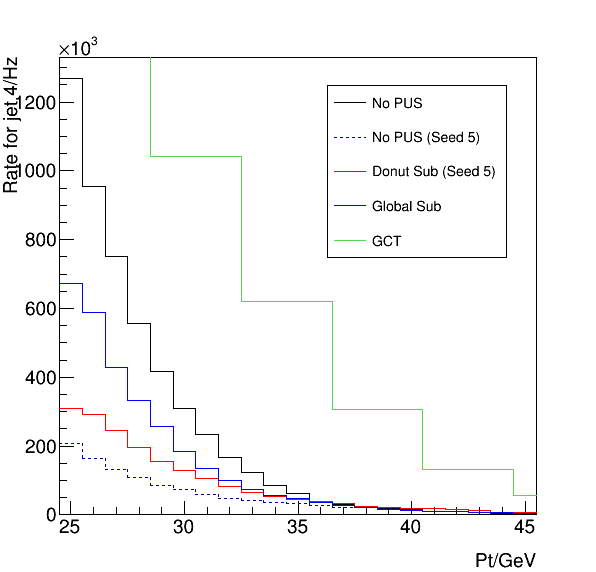
\includegraphics[width=7.2cm]{./Figures/triggerUpgrade/rate3}}
\hfill
\subfigure[Jet 1 Rate vs Number of Interactions \label{fig:label:ratenvtx}]{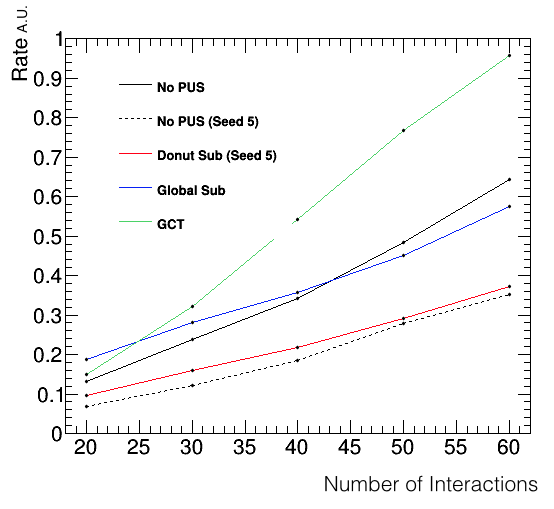
\includegraphics[width=7cm]{./Figures/triggerUpgrade/neutrinonvtx_jet1}}
\caption{In \ref{fig:label:ratejet1} the rate for the 4th jet against threshold is shown. This is reduced for stage 2 compared to GCT and for pileup subtraction. The dependence of the rate at $p_T=30GeV$ for the lead jet with on the number of interactions is shown in figure \ref{fig:label:ratenvtx}}.
\label{fig:label:rates}
\end{figure}
\begin{figure}
\centering
    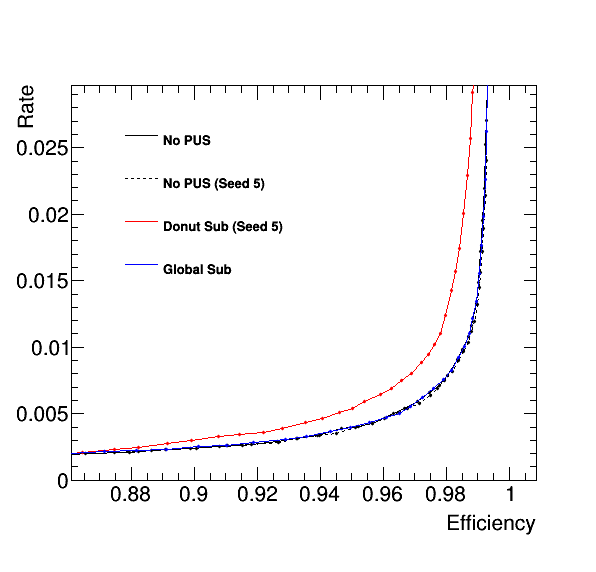
\includegraphics[width=8cm]{././Figures/triggerUpgrade/jet1RateEff}
  \caption{Rate versus efficiency for lead jet. Performance is consistent except for donut which appears to excessively reduce efficiency}
  \label{fig:label:rateeff}
\end{figure}
\subsection{Turn On Plots}
To benchmark the performance of the L1 jets their $p_T$ must be compared with matched generator level quantities. To do this the generator level quantity is plotted with a cut on the matched L1 quantity (the turn on). This is shown in figure \ref{turnon} for the 4th jet. The stage 2 quantities are shown to be very comparable, however, the   GCT is less sharp and thus the agreement with gen worse. 
\begin{figure}
\centering
    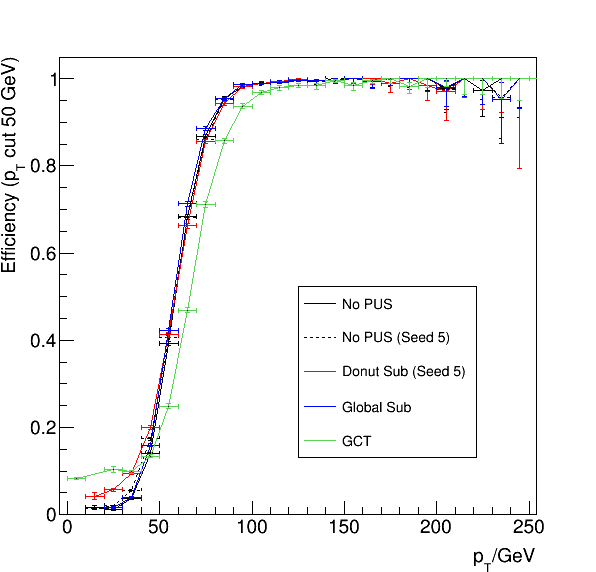
\includegraphics[width=7.5cm]{./Figures/triggerUpgrade/turnon3_50}
  \caption{Turn on curve for the 4th jet at 50 GeV showing comparable behaviour for the stage 2 quantities and a shallower turn on for GCT.}
  \label{turnon}
\end{figure}
\subsection{Energy Sums}
Lastly, the energy sums, \scalht and \mht~, were investigated. To nullify the problem of the lower calibration limit, only jets above this are included in the sums. This also has the effect of removing the majority of remaining clustered pileup jets. Pileup is expected to be approximately uniform and so should not affect the missing energy in the event. The results for a $t\bar{t}$ sample are shown in figure \ref{fig:label:sums}. Pileup subtraction improves the agreement as compared to gen.  The \scalht shows especially good agreement with gen for the case of a seed as compared to global $\rho$. This is due to the under subtraction bias of this method. The \mht shows similar levels of agreement for all cases as expected. 
\begin{figure}
\hfill
\subfigure[\scalht\label{fig:label:ht}]{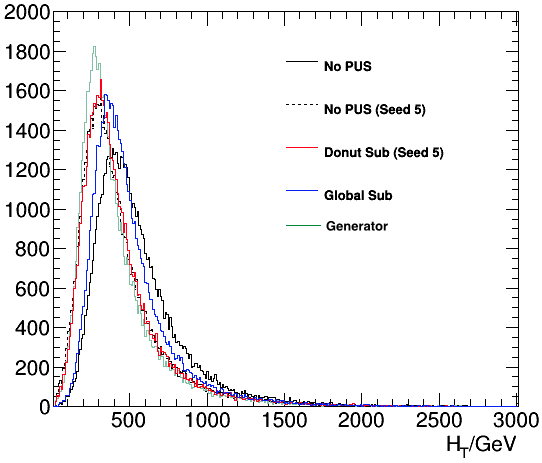
\includegraphics[width=7cm]{./Figures/triggerUpgrade/ht_ttbar}}
\hfill
\subfigure[\mht~\label{fig:label:mht}]{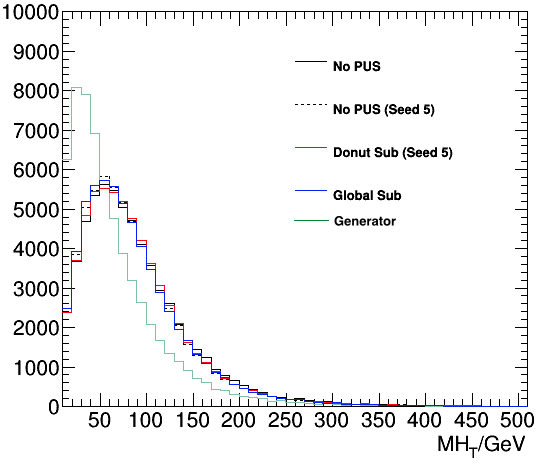
\includegraphics[width=7cm]{./Figures/triggerUpgrade/mht_ttbar}}
\caption{In figure \ref{fig:label:ht} the total energy shows good agreement with the generator level quantity. This is improved by requiring a seed threshold. In figure \ref{fig:label:mht} similar agreement is shown for all cases}
\label{fig:label:sums}
\end{figure}
\section{Conclusions}
The jet algorithm has been shown to give very compatible results with the offline anti-kT algorithm and maintain a high matching efficiency to generator level quantities.  Pileup subtraction has been shown to be important for  run 2. While both global and donut subtraction have been shown to flatten the response against number of interactions (\ref{fig:label:resolution}) each has weaknesses that must be addressed. Figure \ref{fig:label:rateeff} shows that applying a seed threshold is comparable to global subtraction at killing rate while maintaining efficiency. Donut subtraction appears to perform less well than applying the seed threshold alone. This may be due to the susceptibility to fluctuations and contamination. Further studies are underway to increase the sampling area for donut subtraction which is expected to improve performance. Figure \ref{fig:label:sums} shows global $\rho$ overestimating the $H_T$. This is due to the under-subtraction bias leading to excess energy being left in the event. This may be correcting by applying a seed threshold as for donut but calculating $\rho$ using all jets. 

Further studies are currently underway to utilise the $\eta$ dependence of the pileup in the detector.  The seed threshold applied may be altered depending on the location of the tower to further reduce rate in areas of high pileup while maintaining efficiency in low pileup regions. Improving calibrations such that lower energy jets may be utilised is also key. Finally, increasing the sample size to use $3\times3$ towers for the seed should improve discrimination between pileup and boosted jets. 
